\section{Kalman Filters}
Traditionally, the Kalman Filter (KF) is a tool used to analyse a set of linear data points for an unknown dynamic model. Each data point is passed in 1-by-1 to the filter (thus the k$^{th}$ step involves the k$^{th}$ data point) using the following nomenclature:\newline

$x_{k|k}$ [nx1]:    the k$^{th}$ estimated state space given the first k observations \newline
$x_{k+1|k}$ [nx1]:  the k+1$^{st}$ estimated state space given the first k observations\newline
$F_{k}$ [nxn]:  the state transition function\newline
B_k = ?
U_k = ?\newline
$P_{k|k}$ [nxn]:  the error covariance matrix (the confidence in) $x_{k|k}$\newline
Q [nxn]:    the processing noise (confidence in obervations)\newline
$H_{k}$ [1xn]: the observation model at step k\newline
$z_{k}$ [1x1]: the observation at step k\newline
$y_{k}$ [1x1]: the estimate residual at step k\newline
R [1x1]: the measurement noise (confidence in the predictions)\newline
$S_{k}$ [1x1]: the innovation covariance\newline
$K_{k}$ [nx1]: the kalman gain\newline

Assuming a state space with n parameters, each of these is a matrix with dimensions [AxB] meaning it has A rows and B columns. There exists a proper pairing of Q and R for each dataset, however, they are usually not known. They represent artifacts of the Kalman filters' assumptions. Q is the covariance matrix of a multivariate normal distribution with mean 0 for the variability in each of the n parameters in $x_{k} \forall k$. R is the variance of the normal distribution with mean 0 for the variability in $z_{k}$  \forall k.

Given the appropriate values of Q and R, the KF acts as an optimal estimator as it minimizes the Mean Square Error (MSE) of the predicted x. In practice, this can be thought of as nearly equivalent to a recursive weighted least squares (WLS) estimate where Q acts as the forgetting factor for the KF as lambda does in WLS. 

\subsection{Our Application of the Kalman Filter}
Normally, the Kalman Filter is used smooth out noise while maintaining the general form of the original data. As seen in Figure 3.1, the KF takes the set of noisy observations and it able to reconstruct a good approximation of the true function's behavior.

\begin{figure}[h]
\centering
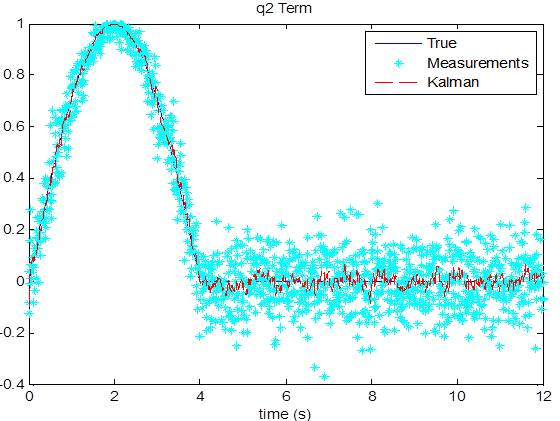
\includegraphics{body/methodology/q2_kalman.jpg}
\caption{Temperary Kalman Filter Picture}
\end{figure}

This traditional usage of the KF iteratively predicts each point value  producing a far less noisy approximation of the true function. We chose to instead use it to approximate the parameters to a function that best fits the trends in the data and from those parameters, forecast for what the value should be in the future. Figure 3.2 shows an example of a line whose parameters were derived using this formulation of the KF.

\begin{figure}[h]
\centering
\includegraphics{body/methodology/example_line.jpg}
\caption{Temp linear Kalman Filter line prediciton}
\end{figure}

We will assume we have some set of noisy linear data in the form (time, value) such that we want to find the best linear approximation of the form 

\begin{equation} Value = \hat{B_{0}} + \hat{B_{1}}*time  \end{equation}

that fits this data. We start with an initial state space estimate of $x_{0|0}$, error covariance matrix estimate $P_{0|0}$ and chosen values of Q and R.

\begin{align}
    x_{0|0} &= \begin{bmatrix}
           B_{0} \\
           B_{1}
         \end{bmatrix}
  \end{align}
  
  The first step is prediction. We calculate $x_{k+1|k}$ and $P_{k+1|k}$ at the next iteration based on the current $x_{k|k}$ and $P_{k|k}$.
  
  \begin{subequations}
  \begin{align}
  \hat{x}_{k+1|k} = F_{k}* \hat{x}_{k|k}+B_{k}u_{k}   \\
  P_{k+1|k} = F_{k}* P_{k|k}*F_{k}^{T}+Q
  \end{align}
  \end{subequations}
  
  For our purposes, we've assumed $F_{k}$ is always identity.
  
  \begin{align}
    F_{k} &= \begin{bmatrix}
           1&0 \\
           0&1
         \end{bmatrix}
         \forall k
  \end{align}
  
  Since any matrix multiplied by identity is always the original matrix, this reduces our prediction equations to the form
  
  \begin{subequations}
  \begin{align}
  \hat{x}_{k+1|k} = \hat{x}_{k|k}+B_{k}u_{k}   \\
  P_{k+1|k} = P_{k|k}+Q
  \end{align}
  \end{subequations}
  
  This is a simplification as we know the true function is not constant. However, by assuming so, we aim to accurately capture the general trend of the data with the goal of producing rather rough forecasting predictions. P represents the confidence (or variability) of each parameter in the current state space with larger values of P meaning less confidence in \hat{x}. From Equ. 3.5b we can see that providing a larger Q causes consistently larger estimates of P. This makes sense as Q is a measure of the variability in each parameter of x, so larger Q's should cause the KF to be less confident in it's predictions.
  
  The second step is updating. Each iteration of the KF utilizes a single data point, so the k$^{th}$ iteration with use the point (Time$_{k}$, Value$_{k}$). We begin by calculating the residual (or error from the k$^{th}$ known observation) for (Time$_{k}$, Value$_{k}$).
  
  \begin{equation}
  \centering
  y_{k} = z_{k} - H_{k}\hat{x}_{k+1|k}
  \end{equation}
  
  Here H$_{k}$ is
  
  \begin{align}
    H_{k} &= \begin{bmatrix}
           1&Time_{k}
         \end{bmatrix}
  \end{align}
  
  From Equ. 3.2, we can see 
  
  \begin{equation}
  \centering
H_{k}\hat{x}_{k+1|k} = B_{0}*1 + B_{1}*Time_{k}
  \end{equation}
  
  Thus, the y$_{k}$ is simply the difference between the prediction of Value$_{k}$ at Time$_{k}$ and the actual observed Value$_{k}$ at Time$_{k}$.
  
  We then perform the innovation step where we calculate S$_{k}$. S$_{k}$ can be understood as a metric for the confidence in observation z$_{k}$ as it represents the variability of all observations thus far. If the values of z tend to vary greatly, S$_{k}$ will increase. If the values of z vary by only small amount, S$_{k}$ will be small.
  
  \begin{equation}
  \centering
s_{k} = R + H_{k}P_{k|k-1}H_{k}^{T}
  \end{equation}